\chapter{Installation et configuration d\textquotesingle iTop sous Windows}
\minitoc
\newpage

L\textquotesingle installation sous Windows présente plusieurs avantages : elle est simple et rapide à mettre en œuvre grâce à XAMPP, et elle est particulièrement adaptée aux tests, aux projets académiques ainsi qu\textquotesingle aux environnements de développement, sans nécessiter de configuration complexe d\textquotesingle un serveur Linux.

\begin{longtable}[]{@{}
  >{\raggedright\arraybackslash}p{(\columnwidth - 0\tabcolsep) * \real{1.0000}}@{}}
\toprule\noalign{}
\endhead
\bottomrule\noalign{}
\endlastfoot
\textbf{Remarque :} Pour un environnement de production, il est généralement recommandé d\textquotesingle installer iTop sur un serveur Linux (Ubuntu, Debian ou Red Hat), qui offre de meilleures performances, une sécurité renforcée et une maintenance plus facile. \\
\end{longtable}

\section{Étape 1 -- Installation de XAMPP}

Les étapes suivies pour l\textquotesingle installation de XAMPP sont les suivantes :

\begin{itemize}
\item
  Téléchargement de XAMPP depuis le site officiel
\item
  Installation de XAMPP
\item
  Lancement du XAMPP Control Panel
\item
  Démarrage des services Apache et MySQL
\end{itemize}

\subsection{Vérification de l\textquotesingle installation via l\textquotesingle invite de commandes}

Il est possible de vérifier l\textquotesingle installation de XAMPP de plusieurs façons à l\textquotesingle aide de l\textquotesingle invite de commandes (CMD).

Pour vérifier l\textquotesingle existence du dossier d\textquotesingle installation :

\begin{longtable}[]{@{}
  >{\raggedright\arraybackslash}p{(\columnwidth - 0\tabcolsep) * \real{1.0000}}@{}}
\toprule\noalign{}
\endhead
\bottomrule\noalign{}
\endlastfoot
dir C:\textbackslash xampp \\
\end{longtable}

Si XAMPP est correctement installé, les dossiers et fichiers suivants doivent apparaître : apache, htdocs, mysql, php et xampp-control.exe.

Les versions des différents composants peuvent ensuite être vérifiées à l\textquotesingle aide des commandes suivantes :

\begin{longtable}[]{@{}
  >{\raggedright\arraybackslash}p{(\columnwidth - 0\tabcolsep) * \real{1.0000}}@{}}
\toprule\noalign{}
\endhead
\bottomrule\noalign{}
\endlastfoot
1. Vérifier PHP

C:\textbackslash xampp\textbackslash php\textbackslash php.exe -v

2. Vérifier Apache

C:\textbackslash xampp\textbackslash apache\textbackslash bin\textbackslash httpd.exe -v

3. Vérifier MariaDB/MySQL

C:\textbackslash xampp\textbackslash mysql\textbackslash bin\textbackslash mysql.exe -\/-version \\
\end{longtable}

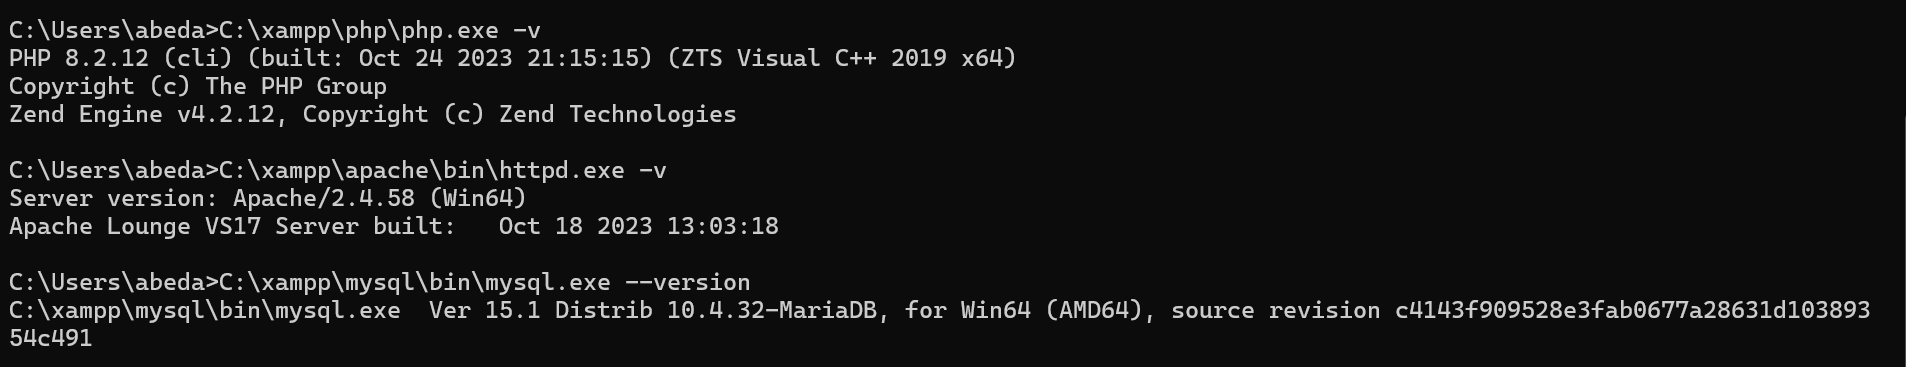
\includegraphics[width=7.68403in,height=1.91042in]{image3.png}

\emph{Figure 1 : Vérification des versions de PHP, Apache et MariaDB via l\textquotesingle invite de commandes}

Une fois Apache et MySQL démarrés, l\textquotesingle accès à phpMyAdmin permet de confirmer le bon fonctionnement de l\textquotesingle environnement :

\begin{longtable}[]{@{}
  >{\raggedright\arraybackslash}p{(\columnwidth - 0\tabcolsep) * \real{1.0000}}@{}}
\toprule\noalign{}
\endhead
\bottomrule\noalign{}
\endlastfoot
http://localhost/phpmyadmin \\
\end{longtable}

L\textquotesingle ouverture correcte de phpMyAdmin confirme que l\textquotesingle environnement XAMPP fonctionne correctement.

\subsection{Remarque --- Conflit de port rencontré avec MySQL}

Lors du démarrage des services depuis le XAMPP Control Panel, MySQL ne parvenait pas à démarrer et affichait le message d\textquotesingle erreur « MySQL shutdown unexpectedly », comme illustré ci-dessous.

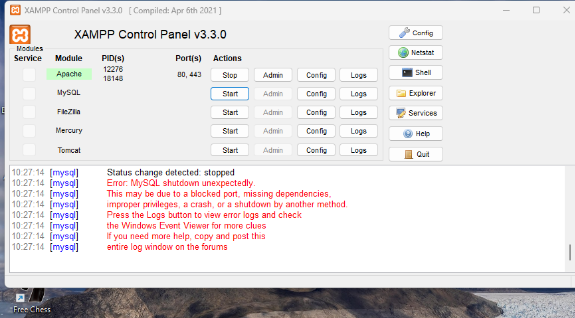
\includegraphics[width=5.3in,height=2.93113in]{image4.png}

\emph{Figure 2 : Message d\textquotesingle erreur affiché par MySQL dans le XAMPP Control Panel}

Une vérification à l\textquotesingle aide de l\textquotesingle utilitaire Netstat a permis d\textquotesingle identifier la cause du problème : le port 3306, utilisé par défaut par MySQL, était déjà occupé par un autre processus mysqld.exe (PID 5756), probablement resté actif suite à une exécution précédente.

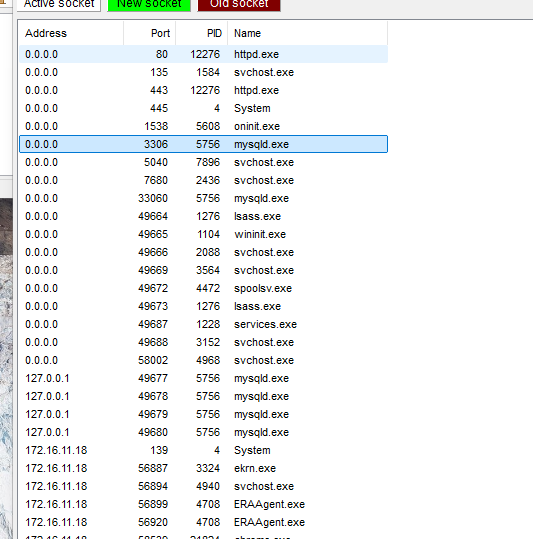
\includegraphics[width=3.6in,height=3.24167in]{image5.png}

\emph{Figure 3 : Vérification du port 3306 déjà utilisé, via Netstat}

Sur les conseils de l\textquotesingle encadrant, il a été choisi de ne pas arrêter ce processus mais de reconfigurer MySQL afin qu\textquotesingle il utilise un autre port. Le fichier de configuration my.ini de XAMPP a ainsi été modifié pour remplacer le port 3306 par le port 3307 :

\begin{longtable}[]{@{}
  >{\raggedright\arraybackslash}p{(\columnwidth - 0\tabcolsep) * \real{1.0000}}@{}}
\toprule\noalign{}
\endhead
\bottomrule\noalign{}
\endlastfoot
\begin{minipage}[t]{\linewidth}\raggedright
\#port=3306\\
port=3307\strut
\end{minipage} \\
\end{longtable}

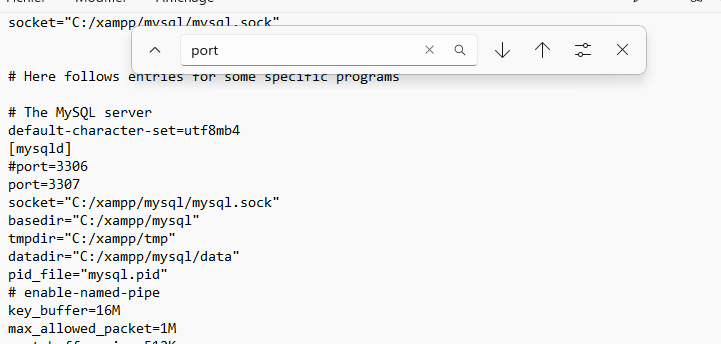
\includegraphics[width=5.5in,height=2.62413in]{image6.png}

\emph{Figure 4 : Modification du port de MySQL dans le fichier my.ini}

Ce changement de port devant également être répercuté au niveau de phpMyAdmin pour que celui-ci continue à se connecter à MySQL, le fichier config.inc.php a été modifié en conséquence :

\begin{longtable}[]{@{}
  >{\raggedright\arraybackslash}p{(\columnwidth - 0\tabcolsep) * \real{1.0000}}@{}}
\toprule\noalign{}
\endhead
\bottomrule\noalign{}
\endlastfoot
\begin{minipage}[t]{\linewidth}\raggedright
\$cfg{[}\textquotesingle Servers\textquotesingle{]}{[}\$i{]}{[}\textquotesingle host\textquotesingle{]} = \textquotesingle127.0.0.1\textquotesingle;\\
\$cfg{[}\textquotesingle Servers\textquotesingle{]}{[}\$i{]}{[}\textquotesingle port\textquotesingle{]} = \textquotesingle3307\textquotesingle;\\
\$cfg{[}\textquotesingle Servers\textquotesingle{]}{[}\$i{]}{[}\textquotesingle connect\_type\textquotesingle{]} = \textquotesingle tcp\textquotesingle;\strut
\end{minipage} \\
\end{longtable}

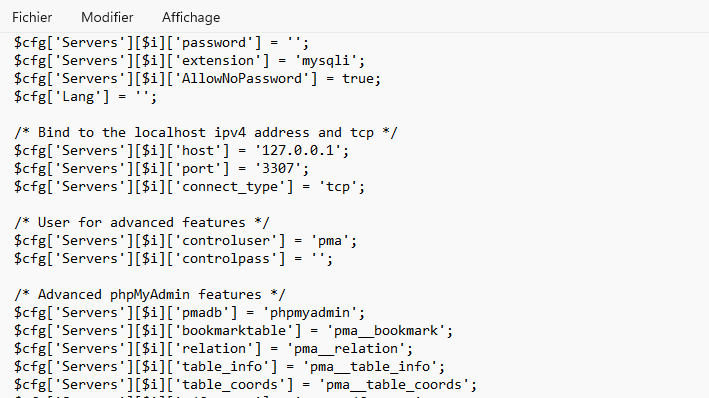
\includegraphics[width=5.5in,height=3.08745in]{image7.png}

\emph{Figure 5 : Mise à jour du port MySQL dans le fichier config.inc.php de phpMyAdmin}

Cette modification a permis à phpMyAdmin de retrouver le service MySQL sur son nouveau port et de fonctionner de nouveau normalement.

\subsection{Récapitulatif de la configuration finale des services}

Après ces ajustements, les différents services utilisés dans le cadre de ce projet fonctionnaient sur les ports suivants :

\begin{longtable}[]{@{}
  >{\raggedright\arraybackslash}p{(\columnwidth - 2\tabcolsep) * \real{0.5000}}
  >{\raggedright\arraybackslash}p{(\columnwidth - 2\tabcolsep) * \real{0.5000}}@{}}
\toprule\noalign{}
\endhead
\bottomrule\noalign{}
\endlastfoot
\textbf{Service} & \textbf{Port} \\
Apache HTTP & 80 \\
Apache HTTPS & 443 \\
MySQL / MariaDB & 3307 \\
\end{longtable}

\section{Étape 2 -- Téléchargement d\textquotesingle iTop}

Le site officiel iTop Hub ne proposant pas un accès direct et clair au téléchargement, la version iTop Community a été récupérée directement depuis la page des fichiers sur SourceForge, qui constitue le dépôt officiel des versions publiées.

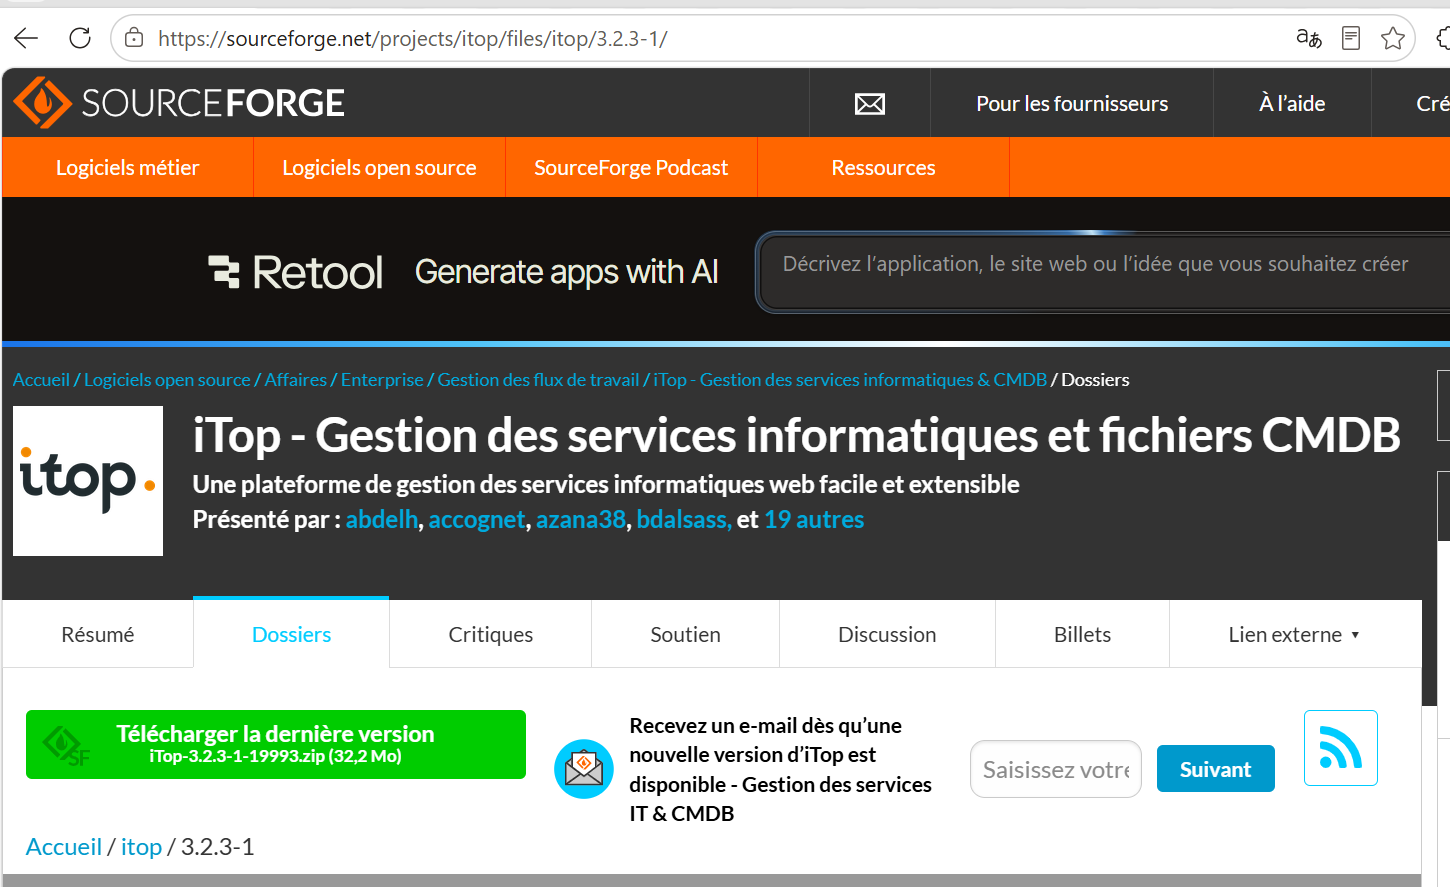
\includegraphics[width=5.49306in,height=2.92708in]{image8.png}

\emph{Figure 6 : Page de téléchargement d\textquotesingle iTop Community sur SourceForge}

Après téléchargement du fichier ZIP et décompression de celui-ci, un dossier nommé \textbf{web} est obtenu, contenant notamment les éléments suivants : index.php, conf/, env-production/, setup/, pages/ et application/. Ce dossier a ensuite été renommé en \textbf{itop}, puis copié dans le répertoire suivant :

\begin{longtable}[]{@{}
  >{\raggedright\arraybackslash}p{(\columnwidth - 0\tabcolsep) * \real{1.0000}}@{}}
\toprule\noalign{}
\endhead
\bottomrule\noalign{}
\endlastfoot
C:\textbackslash xampp\textbackslash htdocs\textbackslash{} \\
\end{longtable}

\section{Étape 3 -- Création de la base de données}

Après démarrage des services Apache et MySQL, l\textquotesingle interface phpMyAdmin a été utilisée pour créer une nouvelle base de données nommée itop, destinée à accueillir les données de l\textquotesingle application.

\begin{longtable}[]{@{}
  >{\raggedright\arraybackslash}p{(\columnwidth - 0\tabcolsep) * \real{1.0000}}@{}}
\toprule\noalign{}
\endhead
\bottomrule\noalign{}
\endlastfoot
http://localhost/phpmyadmin \\
\end{longtable}

\section{Étape 4 -- Lancement de l\textquotesingle installation}

L\textquotesingle installation a ensuite été lancée depuis le navigateur à l\textquotesingle adresse suivante :

\begin{longtable}[]{@{}
  >{\raggedright\arraybackslash}p{(\columnwidth - 0\tabcolsep) * \real{1.0000}}@{}}
\toprule\noalign{}
\endhead
\bottomrule\noalign{}
\endlastfoot
http://localhost/itop \\
\end{longtable}

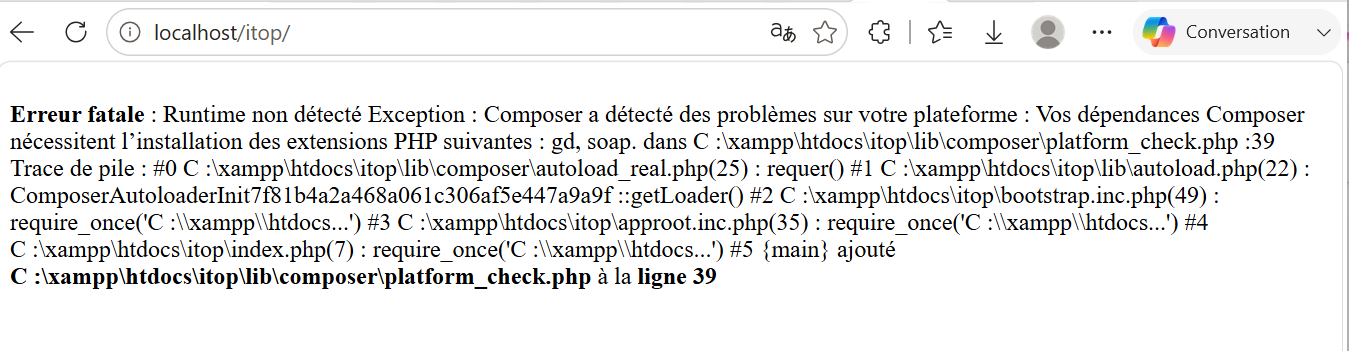
\includegraphics[width=5.47222in,height=1.36806in]{image9.png}

\emph{Figure 7 : Erreur affichée lors du premier lancement de l\textquotesingle installation d\textquotesingle iTop}

Lors du premier lancement, iTop a été correctement détecté, mais l\textquotesingle installation n\textquotesingle a pas pu démarrer en raison de l\textquotesingle absence d\textquotesingle activation de deux extensions PHP requises : gd et soap. L\textquotesingle activation de ces extensions dans XAMPP a donc été nécessaire avant de poursuivre.

\subsection{A\_Configuration des extensions PHP}

L\textquotesingle activation des extensions PHP manquantes s\textquotesingle est effectuée depuis le panneau de configuration de XAMPP (XAMPP Control Panel), en accédant au fichier php.ini via le bouton Config situé à côté d\textquotesingle Apache, puis en sélectionnant PHP (php.ini).

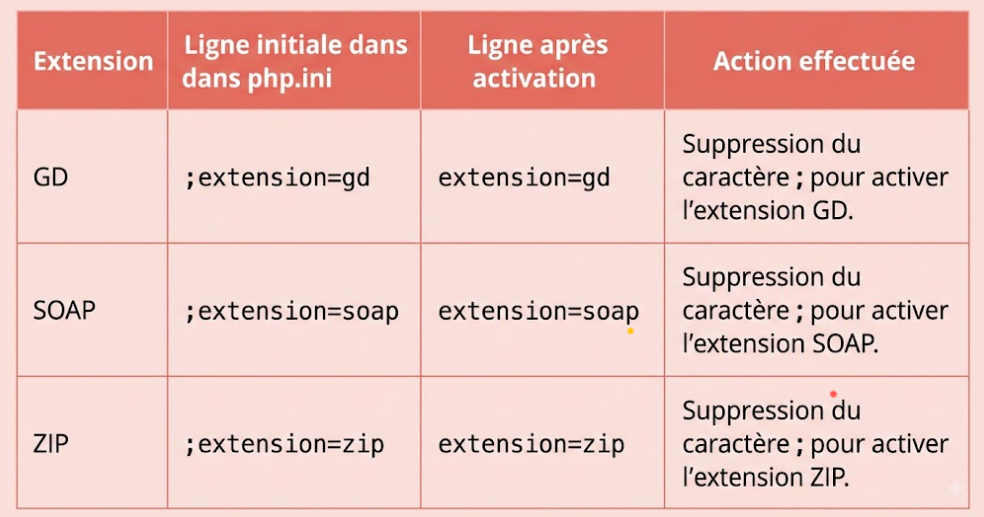
\includegraphics[width=5.10417in,height=2.12083in]{image10.png}

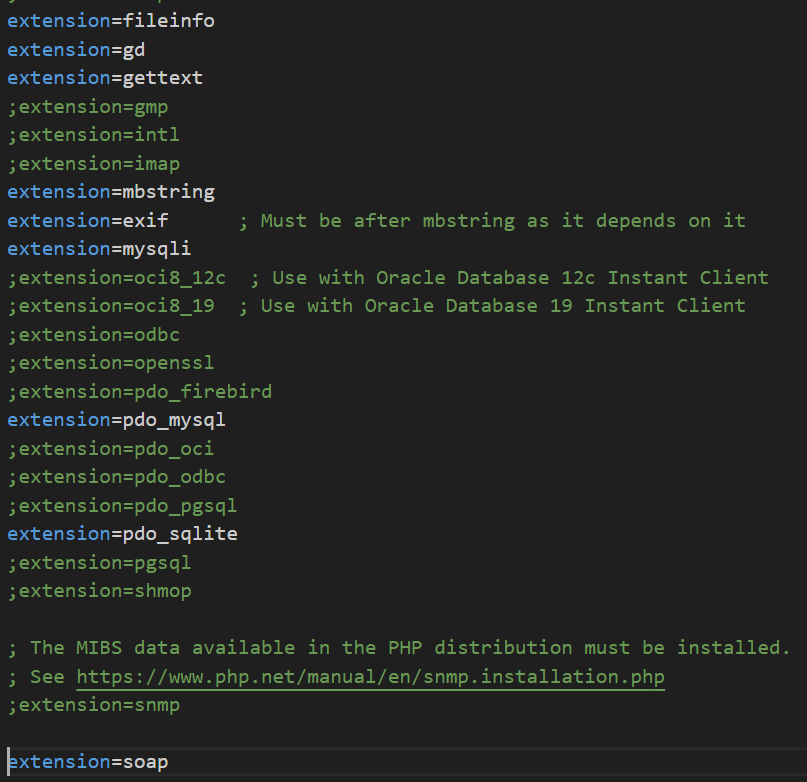
\includegraphics[width=4.16042in,height=2.49306in]{image11.png}

\emph{Figure 8 : Activation des extensions PHP dans le fichier php.ini}

\section{B\_Vérification de la présence du fichier php\_zip.dll}

Afin de confirmer la disponibilité de l\textquotesingle extension ZIP, l\textquotesingle existence du fichier php\_zip.dll a été vérifiée dans le répertoire suivant :

\begin{longtable}[]{@{}
  >{\raggedright\arraybackslash}p{(\columnwidth - 0\tabcolsep) * \real{1.0000}}@{}}
\toprule\noalign{}
\endhead
\bottomrule\noalign{}
\endlastfoot
C:\textbackslash xampp\textbackslash php\textbackslash ext \\
\end{longtable}

La présence de ce fichier confirme que l\textquotesingle extension peut être correctement chargée par PHP.

Après redémarrage du service Apache, l\textquotesingle accès à l\textquotesingle adresse http://localhost/itop a été de nouveau testé, confirmant la disparition de l\textquotesingle erreur initiale liée aux extensions PHP manquantes.

\section{Étape 5 -- Finalisation de l\textquotesingle installation et prise en main de l\textquotesingle interface}

Une fois les extensions PHP gd, soap et zip correctement activées, l\textquotesingle assistant d\textquotesingle installation a pu se poursuivre normalement. L\textquotesingle étape suivante a consisté à configurer l\textquotesingle accès à la base de données : le nom du serveur (localhost), l\textquotesingle identifiant de connexion (root) ainsi que la base de données itop créée précédemment via phpMyAdmin ont été renseignés, comme illustré ci-dessous.

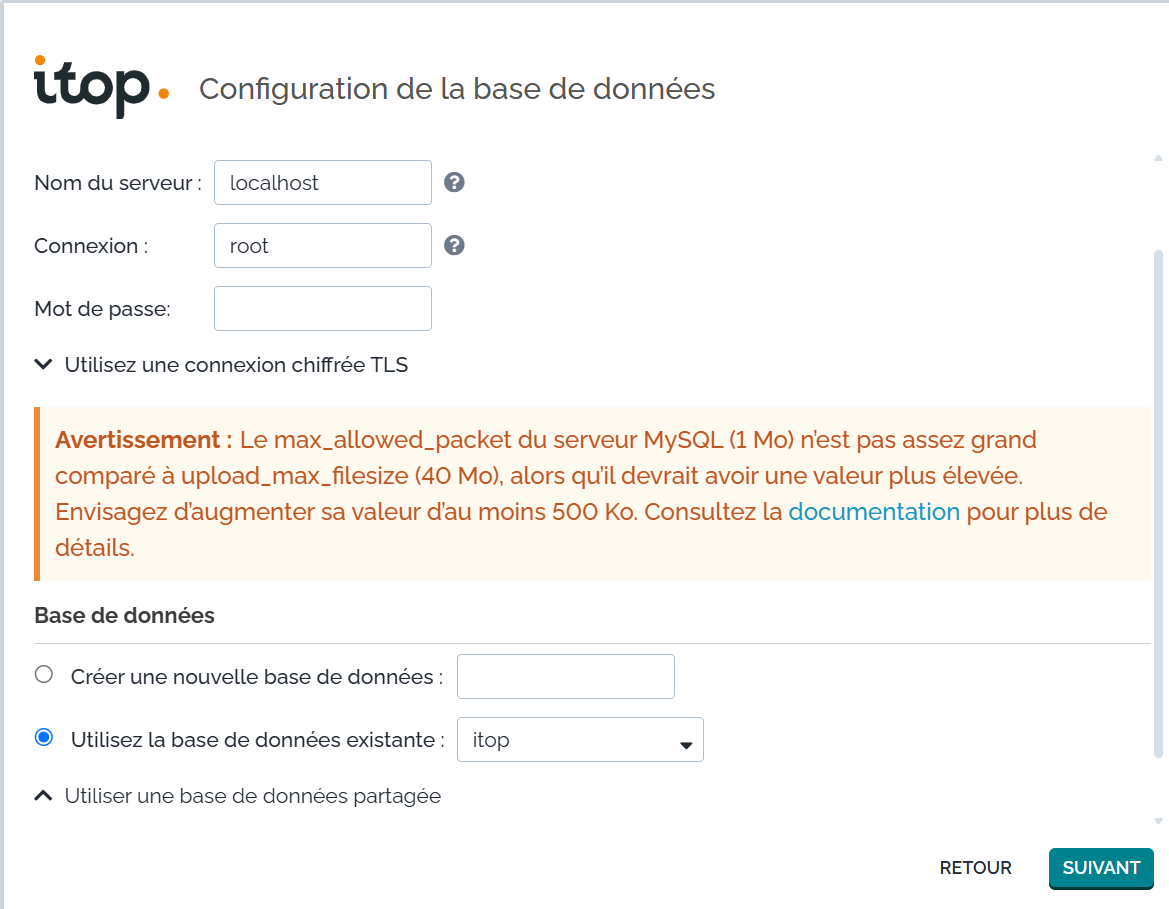
\includegraphics[width=4.75139in,height=2.85694in]{image12.png}

\emph{Figure 9 : Configuration de l\textquotesingle accès à la base de données lors de l\textquotesingle installation}

\subsection{Remarque --- Mise à jour de la configuration d\textquotesingle iTop après changement de port}

Le port de MySQL ayant été modifié dans XAMPP (voir l\textquotesingle Étape 1), il fallait également en tenir compte au niveau de l\textquotesingle assistant d\textquotesingle installation d\textquotesingle iTop : le champ « Nom du serveur » ne pouvait plus se limiter à localhost et devait désormais préciser le nouveau port, sous la forme suivante :

\begin{longtable}[]{@{}
  >{\raggedright\arraybackslash}p{(\columnwidth - 0\tabcolsep) * \real{1.0000}}@{}}
\toprule\noalign{}
\endhead
\bottomrule\noalign{}
\endlastfoot
Server Name : 127.0.0.1:3307 \\
\end{longtable}

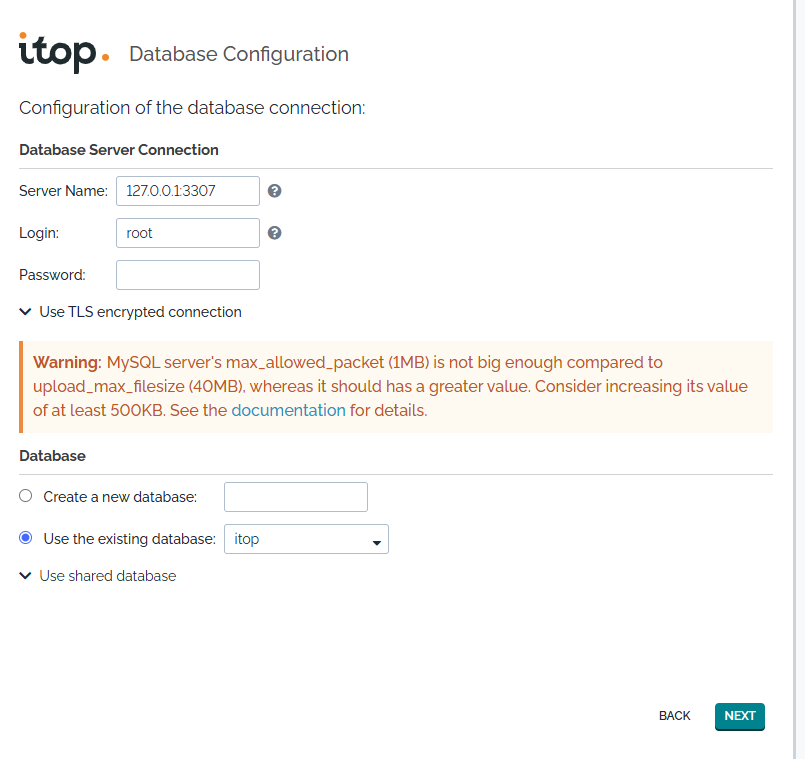
\includegraphics[width=4.00833in,height=3.77847in]{image13.png}

\emph{Figure 10 : Configuration de la base de données avec le port MySQL mis à jour (127.0.0.1:3307)}

Cette correction a permis à iTop de se connecter correctement à MySQL après le changement de port, et l\textquotesingle installation a pu se poursuivre normalement.

L\textquotesingle assistant a ensuite proposé la création du compte administrateur de la plateforme. Un identifiant de connexion (admin), un mot de passe sécurisé ainsi que la langue de l\textquotesingle interface ont été définis à cette étape, comme le montre la figure suivante.

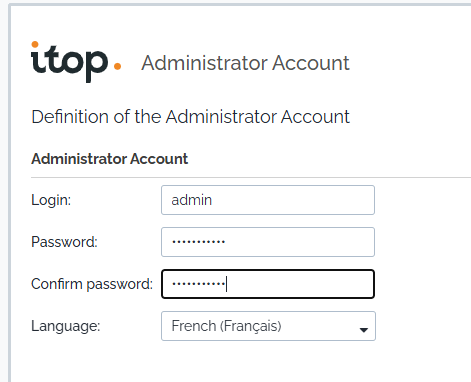
\includegraphics[width=3.35625in,height=2.19514in]{image14.png}

\emph{Figure 11 : Création du compte administrateur d\textquotesingle iTop (}Motpasse : ma*****6 \emph{)}

Après validation de ces paramètres, iTop a terminé son installation et a automatiquement ouvert une session avec le compte administrateur créé. Un écran de bienvenue s\textquotesingle est alors affiché, présentant les principales nouveautés de la version 3.2 (newsroom, centre de notifications, accessibilité de l\textquotesingle interface, etc.).

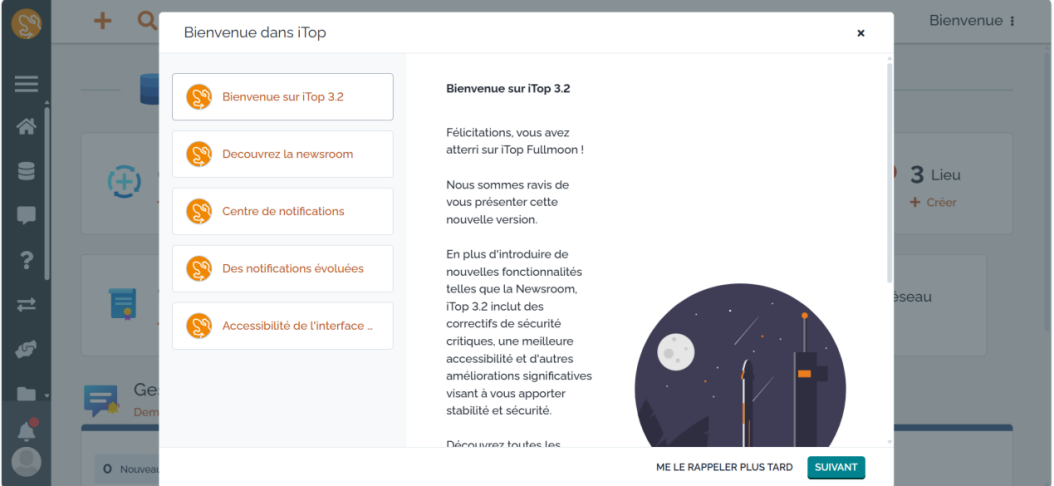
\includegraphics[width=4.79167in,height=2.20833in]{image15.png}

\emph{Figure 12 : Écran de bienvenue affiché lors de la première connexion à iTop}

Après fermeture de cet écran, l\textquotesingle interface principale d\textquotesingle iTop est apparue, confirmant la réussite complète de l\textquotesingle installation. Le tableau de bord affiche notamment le nombre d\textquotesingle éléments de configuration (CIs) déjà présents dans la CMDB (serveurs, équipements réseau, contacts, contrats, etc.) ainsi que le module de gestion des demandes, comme le montre la figure ci-dessous.

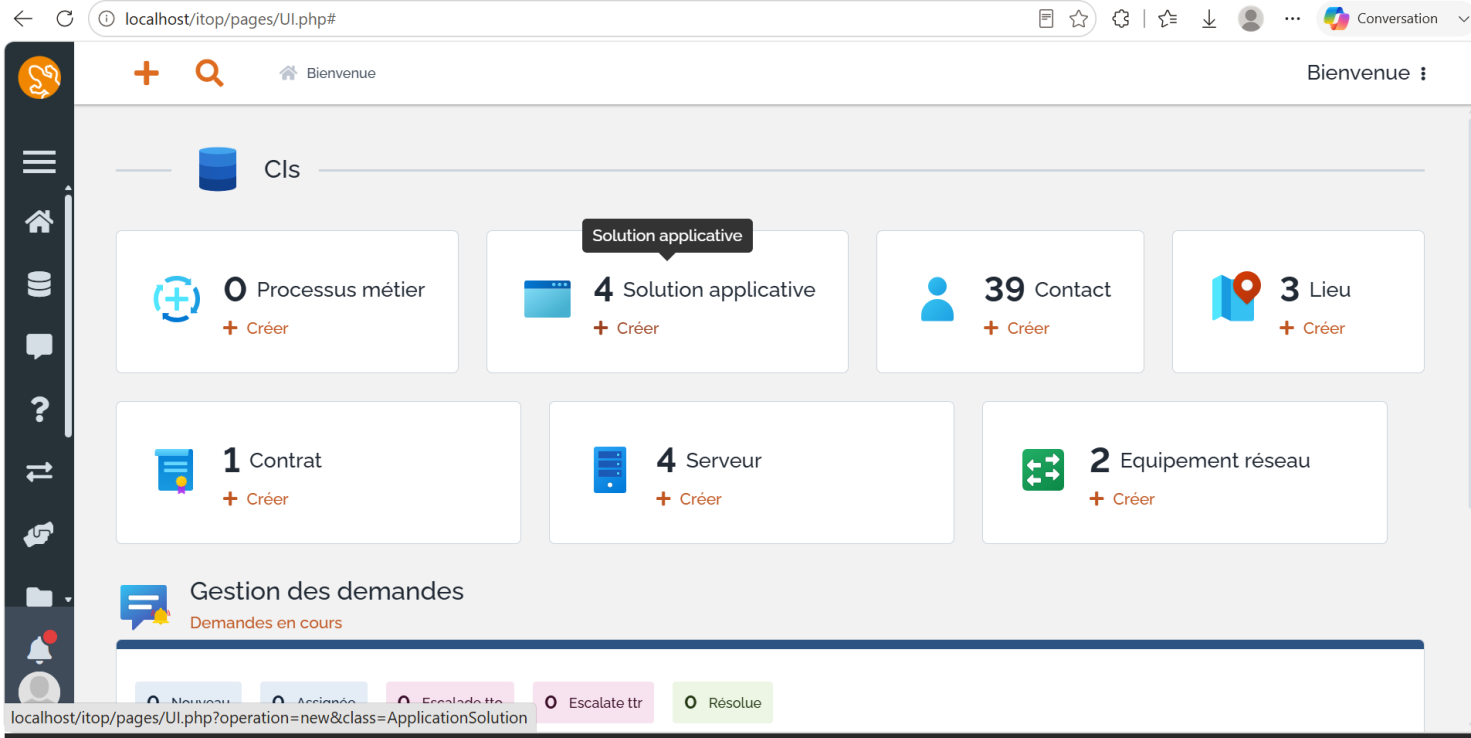
\includegraphics[width=6.6875in,height=3.35278in]{image16.png}

\emph{Figure 13 : Interface principale d\textquotesingle iTop après installation}

Cette dernière étape marque la fin du processus d\textquotesingle installation d\textquotesingle iTop sous Windows : la plateforme est désormais pleinement opérationnelle et prête à être configurée selon les besoins spécifiques du projet mené avec l\textquotesingle APII.


